\documentclass{article}

\usepackage{float}
\usepackage{fancyhdr}
\usepackage{graphicx}
\usepackage{amsmath}
\usepackage{amsfonts}
\usepackage{amssymb}
\usepackage{amsthm}
\usepackage[utf8]{inputenc}
\usepackage[T1]{fontenc}
\usepackage[french]{babel}
\usepackage{libertine}
\usepackage{listings}
\usepackage{color}
\usepackage[table]{xcolor}
\usepackage{minted}
\usepackage{hyperref}
\usepackage{csquotes}
\usepackage{url}
\usepackage[
    backend=biber,
    style=alphabetic,
    sorting=ynt
    ]{biblatex}
\addbibresource{references.bib}

\usepackage[center]{caption}
\hypersetup{
    colorlinks=true,
    pdftitle={PFE - Pluie en Australie},
    }
    
\begin{document}

\newcommand{\HRule}{\rule{\linewidth}{0.5mm}}

\begin{titlepage}
  \begin{sffamily}
  \begin{center}
    \hfill
    
\includegraphics[scale=0.06]{./Images/logoINSARouen.png}~\\[1.5cm]

    \textsc{\LARGE INSA ROUEN}\\[1cm]

    \textsc{\Large Projet de Fin d'Études}\\[1cm]

    \HRule \\[0.4cm]
    { \huge \bfseries Pluie en Australie\\[0.4cm] }

    \HRule \\[1cm]
    %\includegraphics[width=0.7\textwidth]{Ressources/front.pdf}
    %\\[1cm]

    \begin{minipage}{0.4\textwidth}
      \begin{flushleft} \large
        Théophile THIERRY\\
      \end{flushleft}
    \end{minipage}
    \begin{minipage}{0.4\textwidth}
      \begin{flushright} \large
        \textsc{M. PORTIER}\\
         2021-2022\\
      \end{flushright}
    \end{minipage}

    \vfill

  \end{center}
  \end{sffamily}
\end{titlepage}

\tableofcontents
\newpage

\part{Description des données}

\section{Présentation des données}

Les données utilisées pour ce projet peuvent être trouvées sur le site \href{https://www.kaggle.com/jsphyg/weather-dataset-rattle-package}{Kaggle}. Elles ont été récupérées des données du gouvernement australien, dans la partie \href{http://www.bom.gov.au/climate/dwo}{Daily Weather Observations}, et ont été complétées avec les données de la partie :  \href{http://www.bom.gov.au/climate/data}{Climate Data Online}.

Ces données contient 10 années d'observations de la météo australienne sur 49 lieux différents entre 2007 et 2017. Une observation est constituée de (presque) toutes ces variables : 

\begin{itemize}
    \item Date : date de la mesure.
    \item Location : localisation de la mesure.
    \item MinTemp : température minimale dans les 24h jusqu'à 9h du matin (en °C).
    \item MaxTemp : température maximale dans les 24h jusqu'à 9h du matin (en °C).
    \item Rainfall : précipitation dans les 24h jusqu'à 9h du matin (en mm).
    \item Evaporation : bac d'évaporation de classe A dans les 24h jusqu'à 9h du matin (en mm).
    \item Sunshine : ensolleillement en heure dans les 24h jusqu'à minuit.
    \item WindGustDir : direction de la plus forte rafale dans les 24 heures jusqu'à minuit (16 points cardinaux/intercardinaux).   
    \item WindGustSpeed : vitesse de la plus forte rafale dans les 24 heures jusqu'à minuit (16 points cardinaux/intercardinaux).
    \item WindDir9am : direction du vent à 9h du matin.
    \item WindDir3pm : idem mais à 15h.
    \item WindSpeed9am : vitesse du vent à 9h.
    \item WindSpeed3pm : idem à 15h.
    \item Humidity9am : taux d'humidité relative à 9h.
    \item Humidity3pm : idem à 15h.
    \item Pressure9am : pression atmosphérique réduite au niveau moyen de la mer à 9h.
    \item Pressure3pm : idem à 15h.
    \item Cloud9am : fraction du ciel couverte par un nuage à 9h (en huitième).   
    \item Cloud3pm : idem à 15h.
    \item Temp9am : température à 9h (en °C).
    \item Temp3pm : idem à 15h.
    \item RainToday : s'il a plu le jour même.
    \item RainTomorrow : s'il a plu le lendemain.   
\end{itemize}

Jetons tout d'abord un coup d'oeil aux variables numériques de nos données. 

\begin{table}[H]
    \centering
    \begin{tabular}{*{5}{|c}|}
        \hline
        & MinTemp & MaxTemp & Rainfall & Evaporation \\ 
        \hline
        Min. & -8.50 & -4.80 & 0.00 & 0.00 \\ 
        1st Qu. & 7.60 & 17.90 & 0.00 & 2.60 \\ 
        Median & 12.00 & 22.60 & 0.00 & 4.80 \\ 
        Mean & 12.19 & 23.22 & 2.36 & 5.47 \\ 
        3rd Qu. & 16.90 & 28.20 & 0.80 & 7.40 \\ 
        Max. & 33.90 & 48.10 & 371.00 & 145.00 \\ 
        NA's & 1485.00 & 1261.00 & 3261.00 & 62790.00 \\ 
        sd & 6.40 & 7.12 & 8.48 & 4.19 \\ 
        \hline
        \hline
        & Sunshine & WindGustSpeed & WindSpeed9am & WindSpeed3pm \\ 
        \hline
        Min. & 0.00 & 6.00 & 0.00 & 0.00 \\ 
        1st Qu. & 4.80 & 31.00 & 7.00 & 13.00 \\ 
        Median & 8.40 & 39.00 & 13.00 & 19.00 \\ 
        Mean & 7.61 & 40.04 & 14.04 & 18.66 \\ 
        3rd Qu. & 10.60 & 48.00 & 19.00 & 24.00 \\ 
        Max. & 14.50 & 135.00 & 130.00 & 87.00 \\ 
        NA's & 69835.00 & 10263.00 & 1767.00 & 3062.00 \\ 
        sd & 3.79 & 13.61 & 8.92 & 8.81 \\ 
        \hline
    \end{tabular}
\end{table}

Comme nous pouvons le constater, pour certaines d'entre elles, il manque beaucoup d'observations (voir la ligne "NA's"). Nous allons devoir remédier à cela dans les futures parties, et principalement sur les variables \emph{Sunshine} et \emph{Evaporation}, dont nous n'avons respectivement que 52 et 57\% des observations.

Regardons désormais les variables avec des facteurs. Les dates, tout d'abord, vont du 2007-11-01 au 2017-06-25, ce qui représente 3524 jours. 

\begin{figure}[H]
    \centering
    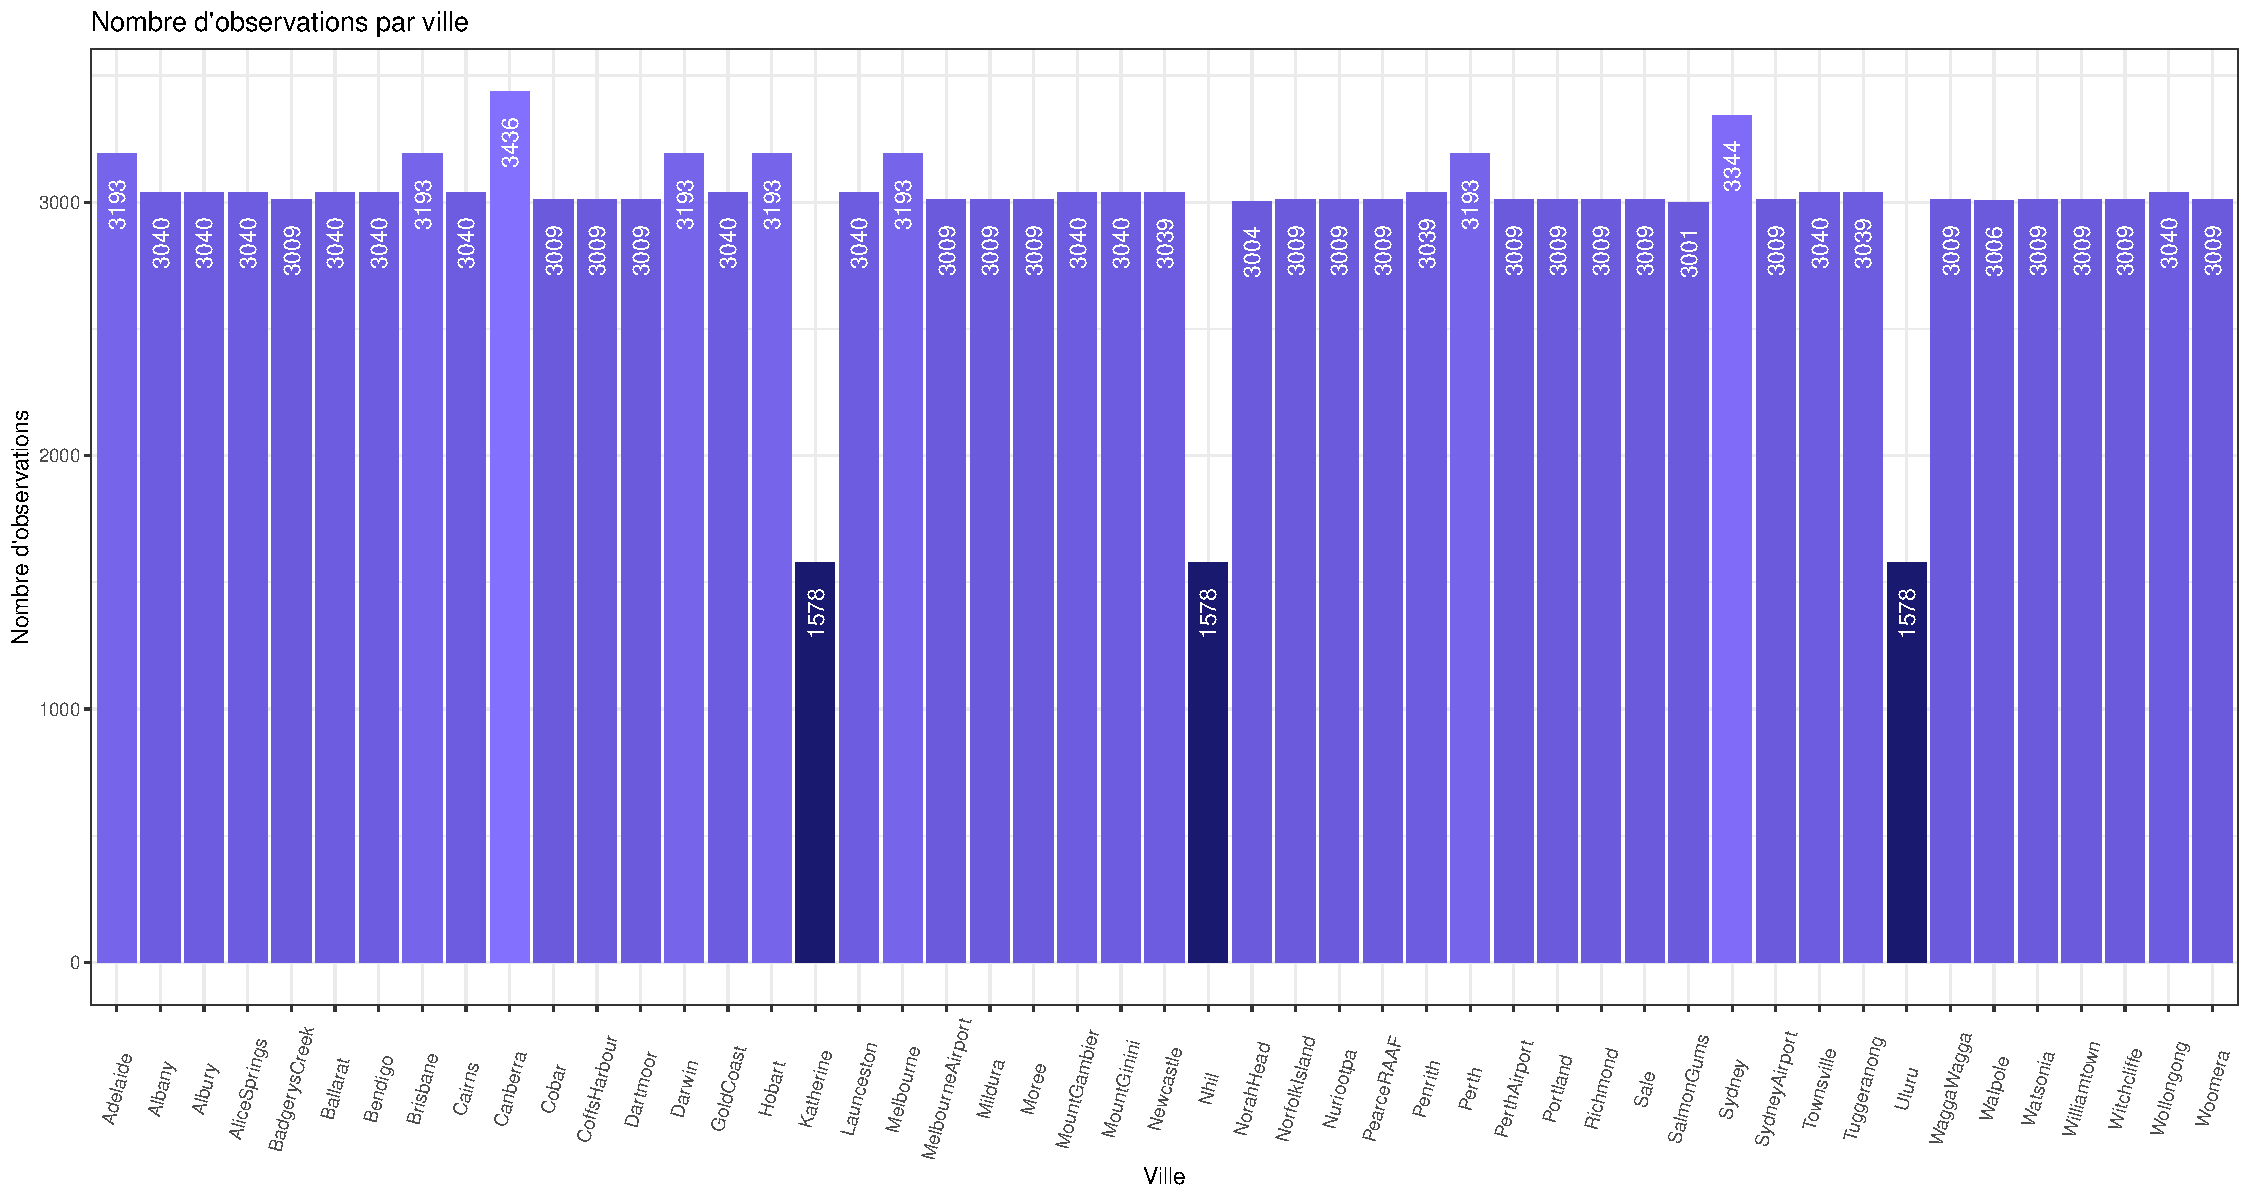
\includegraphics[width=\textwidth]{Images/hist_observations_cities.pdf}
    \caption{Nombre d'observations pour chaque ville}
\end{figure}

On voit déjà qu'il manque certaines dates d'observations pour la plupart des villes, et pour 3 d'entre elles : Katherine, Nhil et Uluru, nous avons moins de la moitié. En regardant de plus près, ceci est dû au fait que les observations démarrent à ces endroits en 2013.

Penchons-nous désormais sur les variables de direction du vent : 

\begin{table}[H]
    \centering
    \resizebox{\textwidth}{!}{
        \begin{tabular}{*{17}{|c}|}
            \hline
            E & ENE & ESE & N & NE & NNE & NNW & NW & S & SE & SSE & SSW & SW & W & WNW & WSW & NA's \\
            \hline
            9181 & 8104 & 7372 & 9313 & 7133 & 6548 & 6620 & 8122 & 9168 & 9418 & 9216 & 8736 & 8967 & 9915 & 8252 & 9069 & 10326 \\
            \hline
        \end{tabular}
    }
    \caption{Variable WindGustDir}
\end{table}

\begin{table}[H]
    \centering
    \resizebox{\textwidth}{!}{
        \begin{tabular}{*{17}{|c}|}
            \hline
            E & ENE & ESE & N & NE & NNE & NNW & NW & S & SE & SSE & SSW & SW & W & WNW & WSW & NA's \\
            \hline
            9176 & 7836 & 7630 & 11758 & 7671 & 8129 & 7980 & 8749 & 8659 & 9287 & 9112 & 7587 & 8423 & 8459 & 7414 & 7024 & 10566  \\
            \hline
        \end{tabular}
    }
    \caption{Variable WindDir9am}
\end{table}
 
\begin{table}[H]
    \centering
    \resizebox{\textwidth}{!}{
        \begin{tabular}{*{17}{|c}|}
            \hline
            E & ENE & ESE & N & NE & NNE & NNW & NW & S & SE & SSE & SSW & SW & W & WNW & WSW & NA's \\
            \hline
            8472 & 7857 & 8505 & 8890 & 8263 & 6590 & 7870 & 8610 & 9926 & 10838 & 9399 & 8156 & 9354 & 10110 & 8874 & 9518 & 4228   \\
            \hline
        \end{tabular}
    }
    \caption{Variable WindDir3pm}
\end{table}

Les 16 niveaux utilisés pour ces variables sont tous représentés, on peut donc considérer cette variable comme un entier allant de 1 à 16. Avec 1 la direction Est et 16 la direction Ouest-Sud-Ouest (dans l'ordre alphabétique). Ici aussi, on remarque qu'il manque plus de  10 000 observations pour les deux premières variables et 4 000 pour la dernière. 

Enfin, nous avons les deux dernières variables : 

\begin{table}[H]
    \centering
    \begin{tabular}{|c|c|c|}
        \hline
            No &    Yes &   NA's \\
        \hline
        110319 &  31880 &   3261 \\
        \hline
    \end{tabular}
    \caption{Variable RainToday}
\end{table}

\begin{table}[H]
    \centering
    \begin{tabular}{|c|c|c|}
        \hline
            No &    Yes &   NA's \\
        \hline
        110316 &  31877 &   3267 \\
        \hline
    \end{tabular}
    \caption{Variable RainTomorrow}
\end{table}

Maintenant que nous connaissons nos variables, nous allons pouvoir les "simplifier" afin de les rendre plus facilement utilisables. 

Dans un premier temps, nous allons transformer les valeurs des points cardinaux des directions de vent avec une valeur de 1 à 16 pour chaque niveau. Au vu de la distribution de ces 16 variables différentes, nous devons toutes les garder. 

Nous allons ensuite remplacer la variable lieu avec une variable de longitude et de latitude, pour des raisons que nous expliquerons dans la section suivante. Ainsi, nous utiliserons la localisation géographique des lieux à la place de leur nom. 

Enfin, nous allons rajouter une variable correspondant aux climats de chaque lieu (on prendra pour cela une carte des climats et on pourra rentrer à la main chaque climat de chaque lieu). Pour ce qui est de la variable date, nous la remplacerons par une variable saison à seulement 4 niveaux. Ce choix sera expliqué dans une partie sur le climat et sur les périodicités. 

\section{Cartographie}

Notre base de donnée comprend donc une variable "Location", qui est une variable qualitative avec le nom du lieu de mesure. Nous en avons 49 différentes, et afin de visualiser un peu mieux ces différents points d'observation, nous voulons les afficher sur une carte. 

Pour cela, nous allons utiliser le paquet R "rnaturalearth", qui nous offre un moyen simple de dessiner nos propres cartes en utilisant le standard WGS84 (World Geodetic System).

\subsection{Un standard de localisation et une projection}

Afin de localiser avec précision un point sur Terre, nous avons besoin d'un standard de localisation. Un standard est basé sur un système de coordonnées géodésique. Il peut utiliser notamment un système de coordonnées en Longitude et Latitude.

\subsubsection{Latitude et Longitude}

Afin d'avoir une coordonnée pour n'importe quel point sur Terre, nous utilisons des coordonnées de Longitude et de Latitude. Ce sont des valeurs exprimées en degré à partir d'un degré 0 de référence.

La Terre ne peut être représentée comme une sphère car cela rendrait les coordonnées trop imprécises par rapport à la réalité. Elle est de plus arrondie aux pôles et c'est pour ces raisons que nous représentons la Terre par un éllipsoïde. 

La Longitude est une coordonnée géographique représentée par une valeur angulaire, expression du positionnement est-ouest d'un point sur Terre \cite{frwiki:188614923}. Tous les points étant situés sur une courbure de l'élipsoïde reliant les pôle Nord et Sud et traversant l'équateur     perpendiculairement ont la même longitude. Une courbure de référence, appelé "méridien" est choisi arbitrairement (le méridien de Greenwich) comme degré 0. Les valeurs de Longitude s'étendent de -180° vers l'ouest à 180° à l'est par rapport à ce méridien. 

La Latitude est une coordonnée similaire mais qui à pour plan de référence l'équateur. Tous les points sur Terre ayant une même latitude forment un cercle dont le plan est parallèle à celui de l'équateur \cite{frwiki:189341688}. 

\begin{figure}[H]
    \centering
    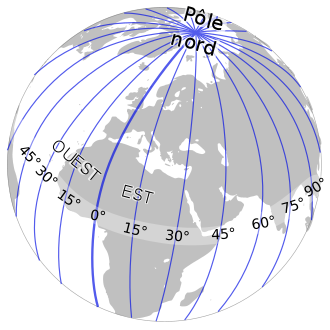
\includegraphics[width=0.3\textwidth]{Images/Cartographie/Longitude.png}
    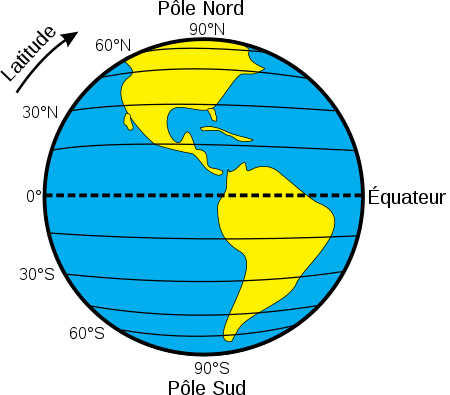
\includegraphics[width=0.3\textwidth]{Images/Cartographie/Latitude.png}
    \caption{Illustration du système de coordonnées de Longitude et Latitude}
\end{figure}

Lorsque l'on combine ce système de coordonnées et une représentation de la Terre en ellipsoïde (au travers de mesures précises des dimensions de la planète), on obtient un système géodésique.

\subsubsection{Le WSG84}

Le World Geodetic System 84 (WGS84) est un système géodésique, et nous pouvons l'utiliser pour nos cartes grâce au paquet "rnaturalearth". Il est notamment utilisé par le système GPS (Global Positioning System). Ce standard à été établi et est maintenu par le National Geospatial Intelligence Agency (NGA) des Etats-Unis \cite{enwiki:1065796786} depuis 1984. Il est basé sur un ellipsoïde de référence raffiné avec le temps pour représenter au mieux la Terre, ainsi que le système de coordonnées en Longitude et Latitude.

Nous avons maintenant un moyen de localiser précisément un point sur Terre grâce à deux valeurs numériques. Pour pouvoir les afficher sur une carte, il nous faut cependant une projection.

\subsubsection{Projections}

La projection cartographique est "un ensemble de techniques permettant de représenter la surface de la Terre dans son ensemble ou en partie sur la surface plane d'une carte" \cite{frwiki:181713838}. La Terre étant sphérique, afin de l'afficher sur une carte plane, il faut la projeter. Il existe différent types de projections, certaines permettent de conserver localement les surfaces, d'autres les angles ou encore les distances sur les méridiens. 

Notre paquet utilise de base une projection dite géographique : elle consiste simplement à prendre les valeurs de latitude et de longitude et des les utiliser comme si elles étaient les coordonnées X et Y (respectivement) d'un repère en deux dimensions. Cette "projection" peut avoir des résultats différents en fonction du système géodésique utilisé. 

Le plus gros inconvénient de cette pratique est la distorsion des surfaces lorsque l'on s'éloigne de l'équateur. Cependant, cela est suffisant dans notre cas, où nous voulons avoir seulement une idée globale de la position des lieux observés des uns par rapport aux autres. De plus, comme nous ne prévoyons pas de mesurer précisément la distance entre deux points, ce système de "projection" géographique est le plus pratique.

\subsection{Affichage sur une carte}

Nous avons désormais tous les éléments pour placer les lieux sur une carte. Le paquet "rnaturalearth" nous permet donc d'avoir une liste de polygone de pays. Le paquet "ozmaps" nous permet d'avoir les polygones des états australiens. Pour les lieux, nous récupérons les latitudes et longitudes manuellement grâce à n'importe quelle base que nous pouvons trouver sur internet et nous les rajoutons à chaque observation en ajoutant deux colonnes. Au final nous pouvons afficher notre carte grâce à ggplot2 : 

\begin{figure}[H]
    \centering
    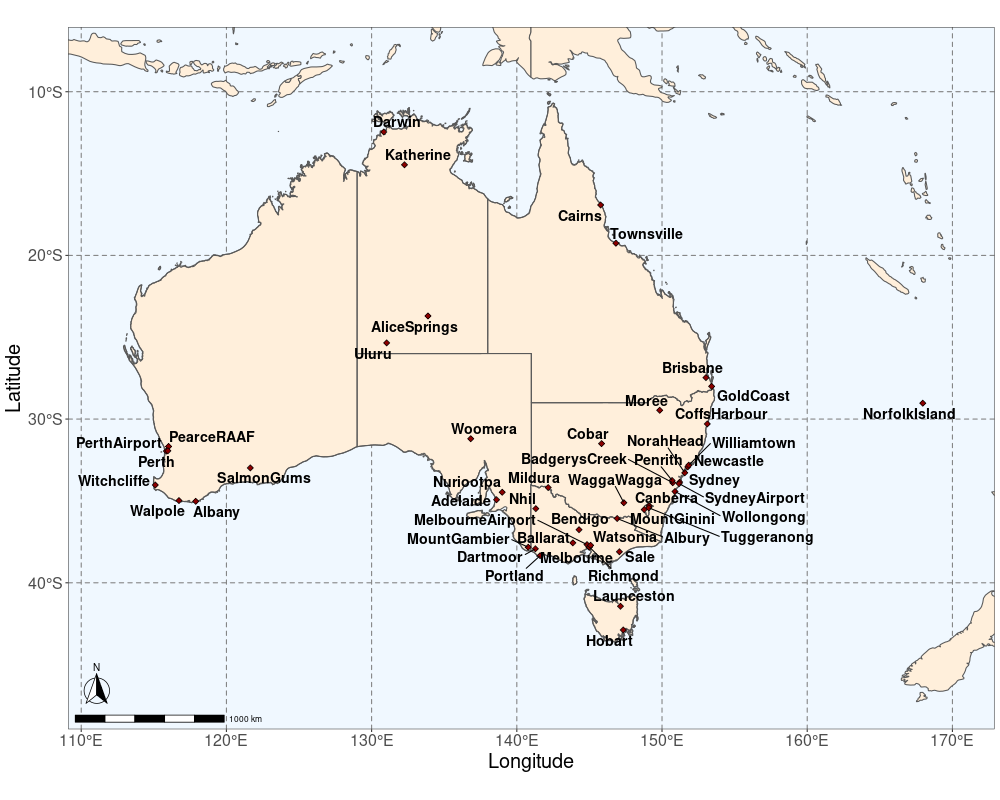
\includegraphics[width=0.8\textwidth]{Images/Cartographie/Australia_full_map.png}
    \caption{Carte de l'Australie et villes dont la météo est observée}
\end{figure}

Nous pouvons desormais utiliser les colonnes de longitude et latitude à la place de la colonne localisation. 

\section{Etude des climats}

Maintenant que nous pouvons afficher les lieux sur une carte, nous pouvons déterminer à quelle zone climatique appartient chaque point.

Comme on peut le voir sur la carte précédente, la plupart des observations ont lieu dans le sud-est du pays, où la concentration d'habitants et de ville est la plus grande. Cette zone correspond à un climat tempéré pour les villes les plus au sud et subtropical pour les villes plus au nord comme Brisbane. Au nord du pays nous avons les villes sur les littoraux dans une zone plus tropicale, et enfin au sud-ouest nous avons d'autre villes subtropicales. Plus à l'intérieur des terres, où il le climat est désertique, nous avons les observations de Uluru, Alice Springs et Woomera. Enfin, nous avons aussi les données de villes sur l'île de Tasmanie et l'île Norfolk. 

\begin{figure}[H]
    \centering
    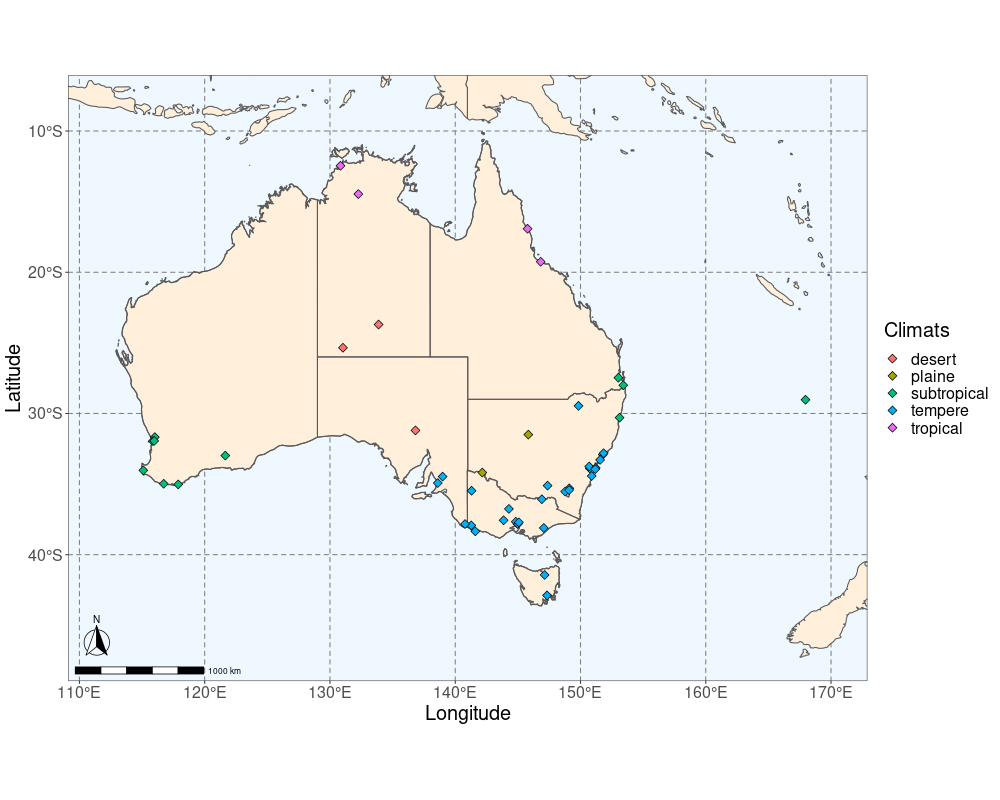
\includegraphics[width=0.8\textwidth]{Images/Cartographie/Australia_climates.png}
    \caption{Carte de l'Australie et climat des villes}
\end{figure}

Nous avons donc les observations de 4 lieux tropicaux, 3 lieux désertiques, 2 lieux dans les plaines (le climat de transition entre désertique et tempéré, en quelques sortes), 11 lieux subtropicaux et enfin 29 lieux tempérés. Certaines données sont liées à des villes mais d'autres à des aéroport ou encore des lieux touristiques.

\subsection{Particularités des climats et périodicité}

Les données étant étalées sur 10 ans, on peut trouver une périodicité dans les mesures à l'année. Nous pouvons alors, pour chaque ville, faire un graphique comprenant les moyennes des température maximales, minimales et moyennes de chaque jour sur 10 ans. Et faire de même pour les précipitations. 

Nous pouvons afficher ces données en fonction des saisons. Nous pourrons ainsi remplacer la variable date par une variable avec uniquement 4 niveaux différents comme expliqué précédemment, à savoir les saisons. Nous prendrons comme saisons : 

\begin{itemize}
    \item L’été, de décembre à février
    \item L’automne, de mars à mai
    \item L’hiver, de juin à août
    \item Le printemps, de septembre à novembre
\end{itemize}


Nous obtenons des graphiques comme suit : 

\begin{figure}[H]
    \centering
    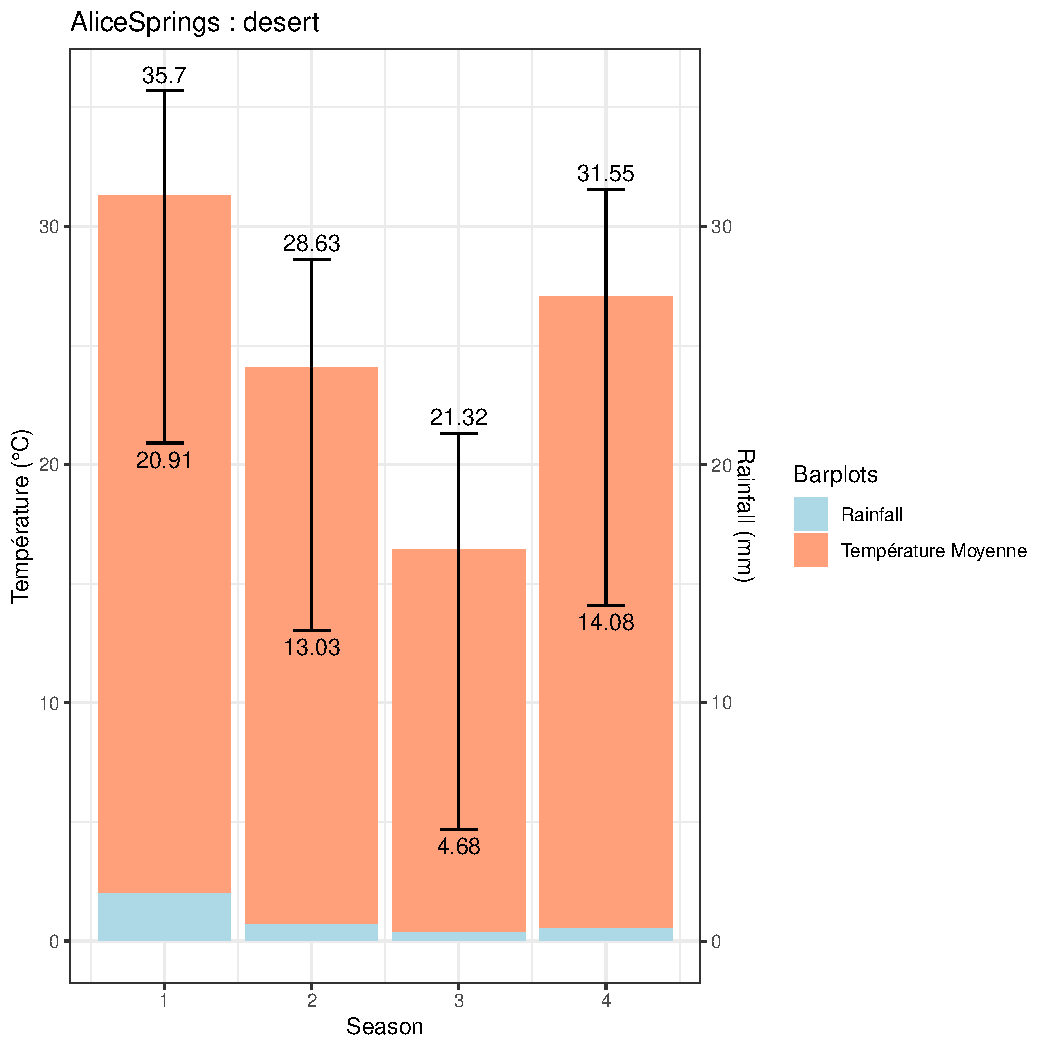
\includegraphics[page=1,width=0.45\textwidth]{Images/Temp_and_Rainfalldesert.pdf}
    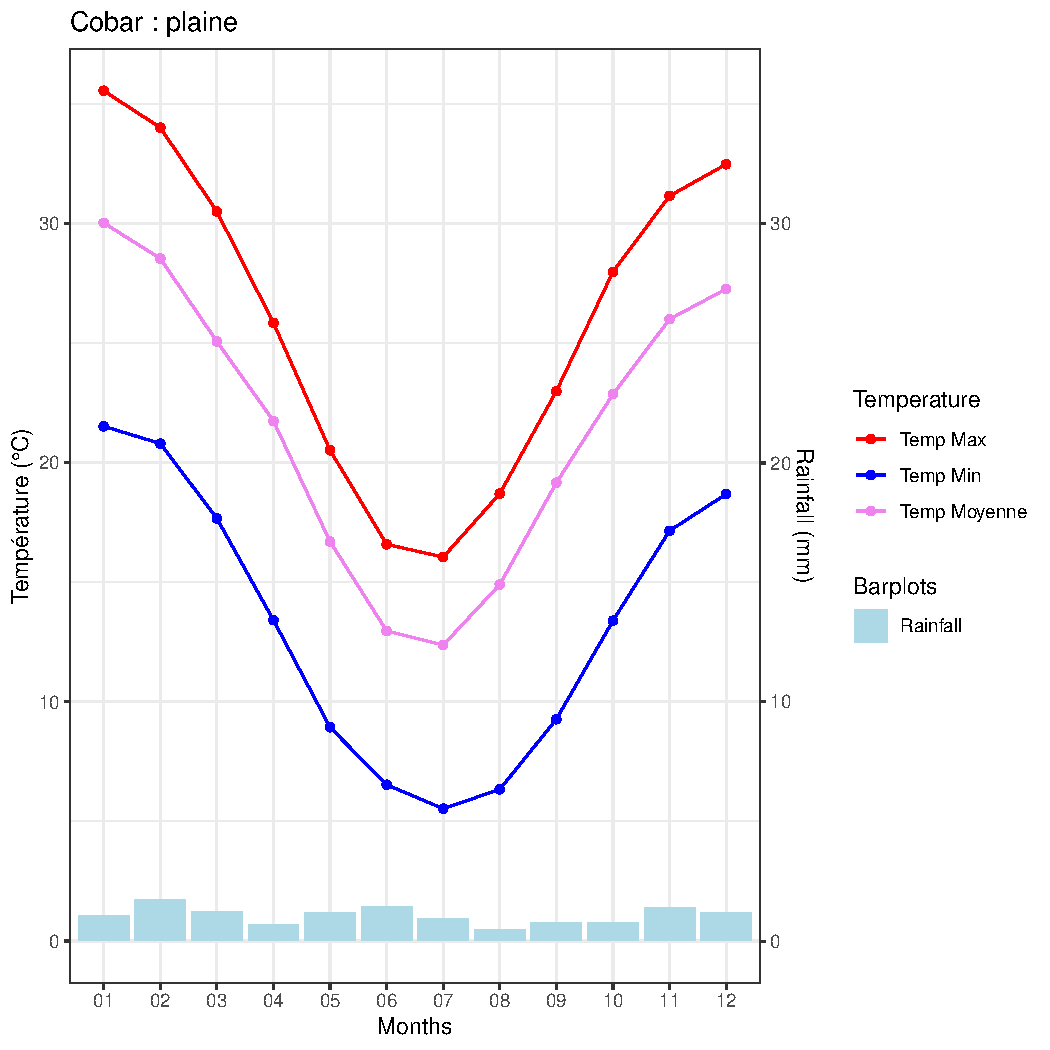
\includegraphics[page=1,width=0.45\textwidth]{Images/Temp_and_Rainfallplaine.pdf}
    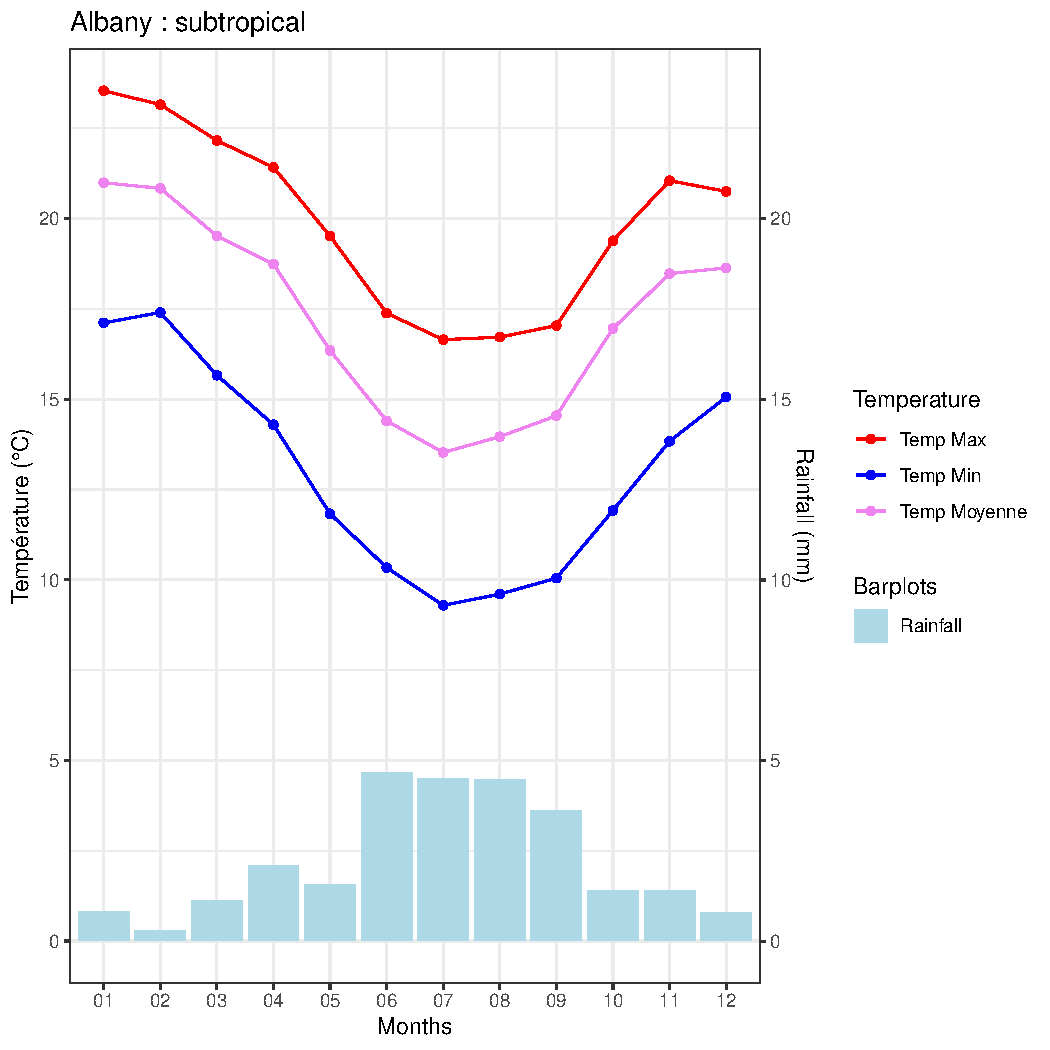
\includegraphics[page=1,width=0.45\textwidth]{Images/Temp_and_Rainfallsubtropical.pdf}
    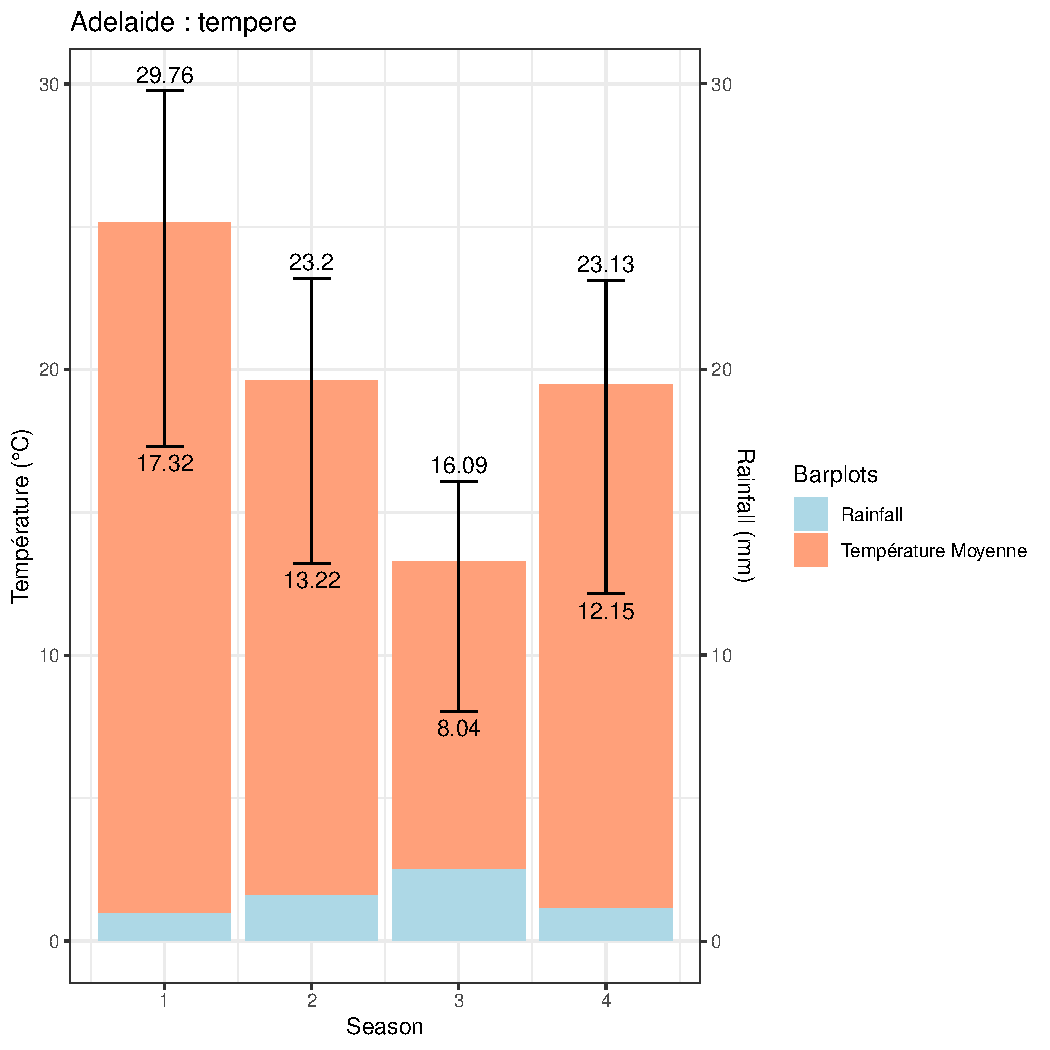
\includegraphics[page=1,width=0.45\textwidth]{Images/Temp_and_Rainfalltempere.pdf}
    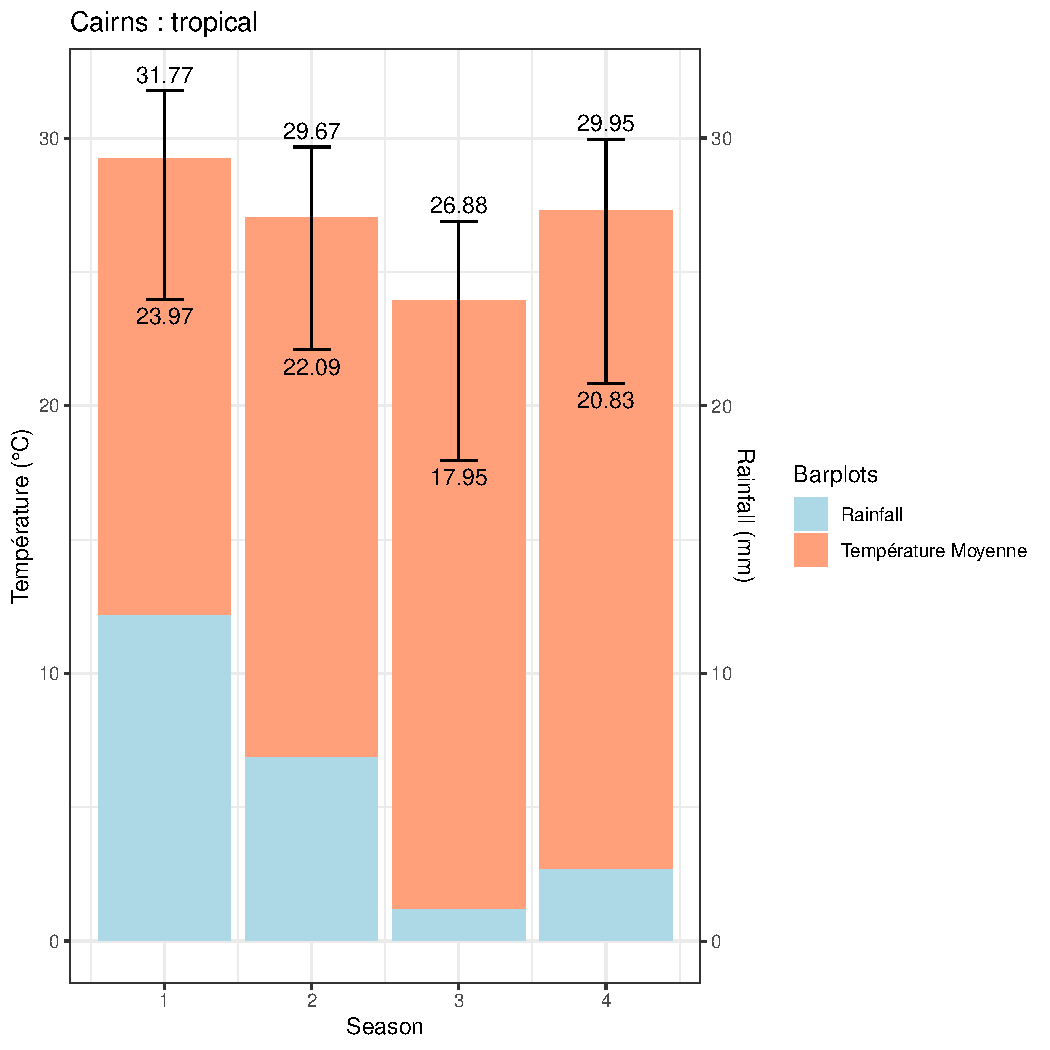
\includegraphics[page=1,width=0.45\textwidth]{Images/Temp_and_Rainfalltropical.pdf}
    \caption{Température Minimale et Maximale ainsi que pluviométrie au cours d'une année pour certaines des villes des données (une par climat)}
\end{figure}

On remarque tout de suite que les températures les plus élevées sont aux alentours de décembre / janvier; l'Australie étant dans l'hémisphère Sud, il s'agit de l'été. 

On remarque ensuite quelques particularité dues aux climats. Dans les régions tempérée et subtropicale tout d'abord, nous avons des températures qui évoluent entre en dessous de 10 degrés et environ 30 degrés, avec en hiver (mai, juin, juillet) plus de pluie que sur le reste de l'année.

Du côté des régions dans les plaines, il pleut moins tout au long de l'année et nous n'observons pas de période de pluie comme pour les deux premières régions. Les températures sont en revanche à peu près les même, voire plus chaudes pendant l'été. Lorsque l'on se penche sur les régions désertiques, les températures sont encore plus hautes et les précipitations sont encore moins importantes, avec seulement quelques millimètres tout au long de l'année. 

A l'opposé, dans les régions tropicales, la température tout au long de l'année évolue moins et reste plus proche de 30 degrés tout au long de l'année (avec une légère baisse en hiver). Dans ces régions, il pleut énormément pendant l'hiver et quasiment pas pendant l'été.

Le choix de ne garder que les saisons et pas les dates se justifie par le fait que si nous voulons prédire s'il pleut le lendemain, nous n'avons pas besoin de savoir précisemment quel jour nous sommes, voire quel mois. On remarque sur les graphiques des différences notables entre les saisons, et celle-ci suffiront sûrement pour nous aider à prédire ce que nous voulons. De plus, nous nous débarassons d'une variable avec beaucoup de facteurs différents, ce qui nous sera bénéfique lors de la mise en place de modèle de prédictions.

Nous nous retrouvons au final avec les variables suivantes : 
\begin{itemize}
    \item MinTemp, MaxTemp
    \item Rainfall
    \item Evaporation
    \item Sunshine
    \item WindGustDir, WindGustSpeed, WindDir9am, WindDir3pm, WindSpeed9am, WindSpeed3pm
    \item Humidity9am, Humidity3pm
    \item Pressure9am, Pressure3pm
    \item Cloud9am, Cloud3pm
    \item Temp9am, Temp3pm
    \item RainToday
    \item RainTomorrow
    \item Season
    \item Latitude, Longitude
    \item Climate
\end{itemize}
Qui sont toutes des variables quantitative ou des variables qualitatives avec moins de 16 niveaux (numérotés en entier).

\section{Complétion des données}

Si l'on regarde les valeurs manquantes, on obtient la distribution suivante : 

\begin{figure}[H]
    \centering
    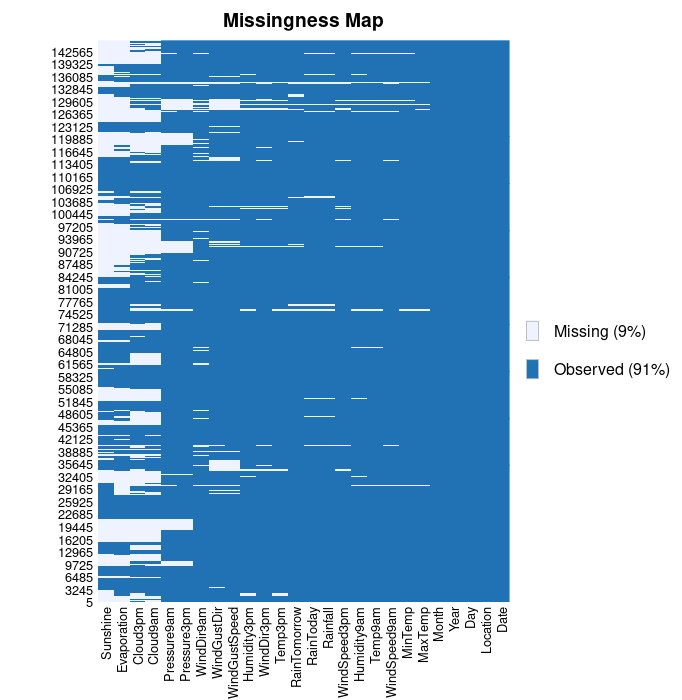
\includegraphics[width=0.7\textwidth]{Images/missmap.png}
    \caption{Missingness Map des données}
\end{figure}

Afin de faire des prédictions sur nos données, nous avons besoin de nous débarasser des observations avec des valeurs \emph{NA}. Pour cela, on utilise la commande \mintinline{R}{na.omit}. On se retrouve avec $56420$ observations sur les $145460$ de base, ce qui est très peu. De plus, la plupart des lieux ne sont plus représentés :

\begin{figure}[H]
    \centering
    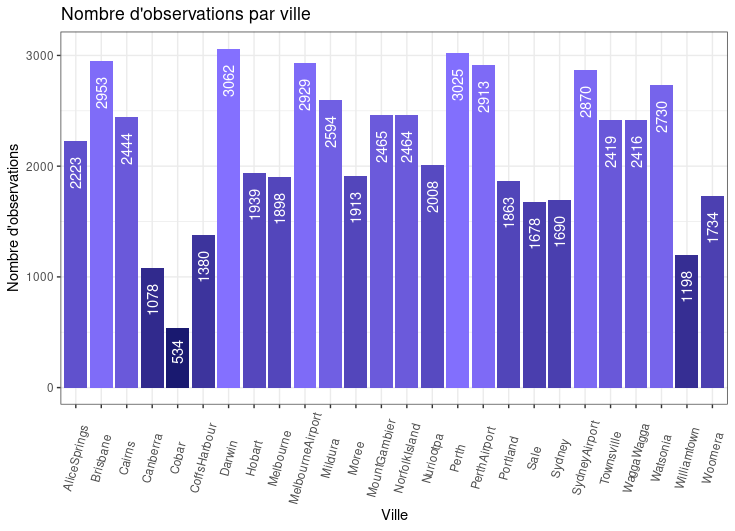
\includegraphics[width=0.7\textwidth]{Images/distribution_lieux_raw.png}
    \caption{Distribution des données après un \emph{na.omit}}
\end{figure}

Nous allons donc chercher un moyen de compléter les valeurs \emph{NA}, et de le faire de façon à ne pas avoir trop de données redondantes et de garder une cohérence vis-à-vis des climats : nous allons copier les données d'une ville à une autre.

Pour cela, nous allons regarder pour chaque variable quels sont les lieux qui ont besoin de complétion, disons les villes qui ont plus de 15\% de \emph{NA} pour cette variable, et quels sont ceux avec lesquels nous pouvons compléter : les autres qui ont plus de 2500 observations. En effet, comme nous l'avons vu, certaines villes n'ont d'observations que sur ~1500 jours. Lorsque nous complétons nos données, nous voulons que les dates coincident pour ne pas perdre en cohérence, ainsi nous voulons compléter les données avec les lieux pour lesquels nous avons des observation sur la période maximale d'observation de notre base de données, soit plus de 2500 jours. 

Lorsque nous copions les données d'un lieu à un autre, nous nous soucions donc de la date d'observation. Cependant, cela ne suffira pas. Nous avons vu en effet que les différents lieux observés appartiennet à des zones climatiques très différentes. Pour chaque variable, nous allons donc associer nos deux listes de lieux (ceux à compléter et ceux avec lesquels compléter) en cherchant les lieux les plus proches de la même zone climatique.

Au final, nous nous retrouvons avec une liste de couples pour chaque variable.

Avec cette méthode, nous allons copier jusqu'à 5 fois maximum les données d'une ville pour une autre ville, et nous le ferons de manière "intelligente", sans perte de cohérence par rapport aux climats des lieux observés. Nous pouvons afficher quelles données de quelles villes vont compléter quelle autre villes sur des cartes comme celle-ci :

\begin{figure}[H]
    \centering
    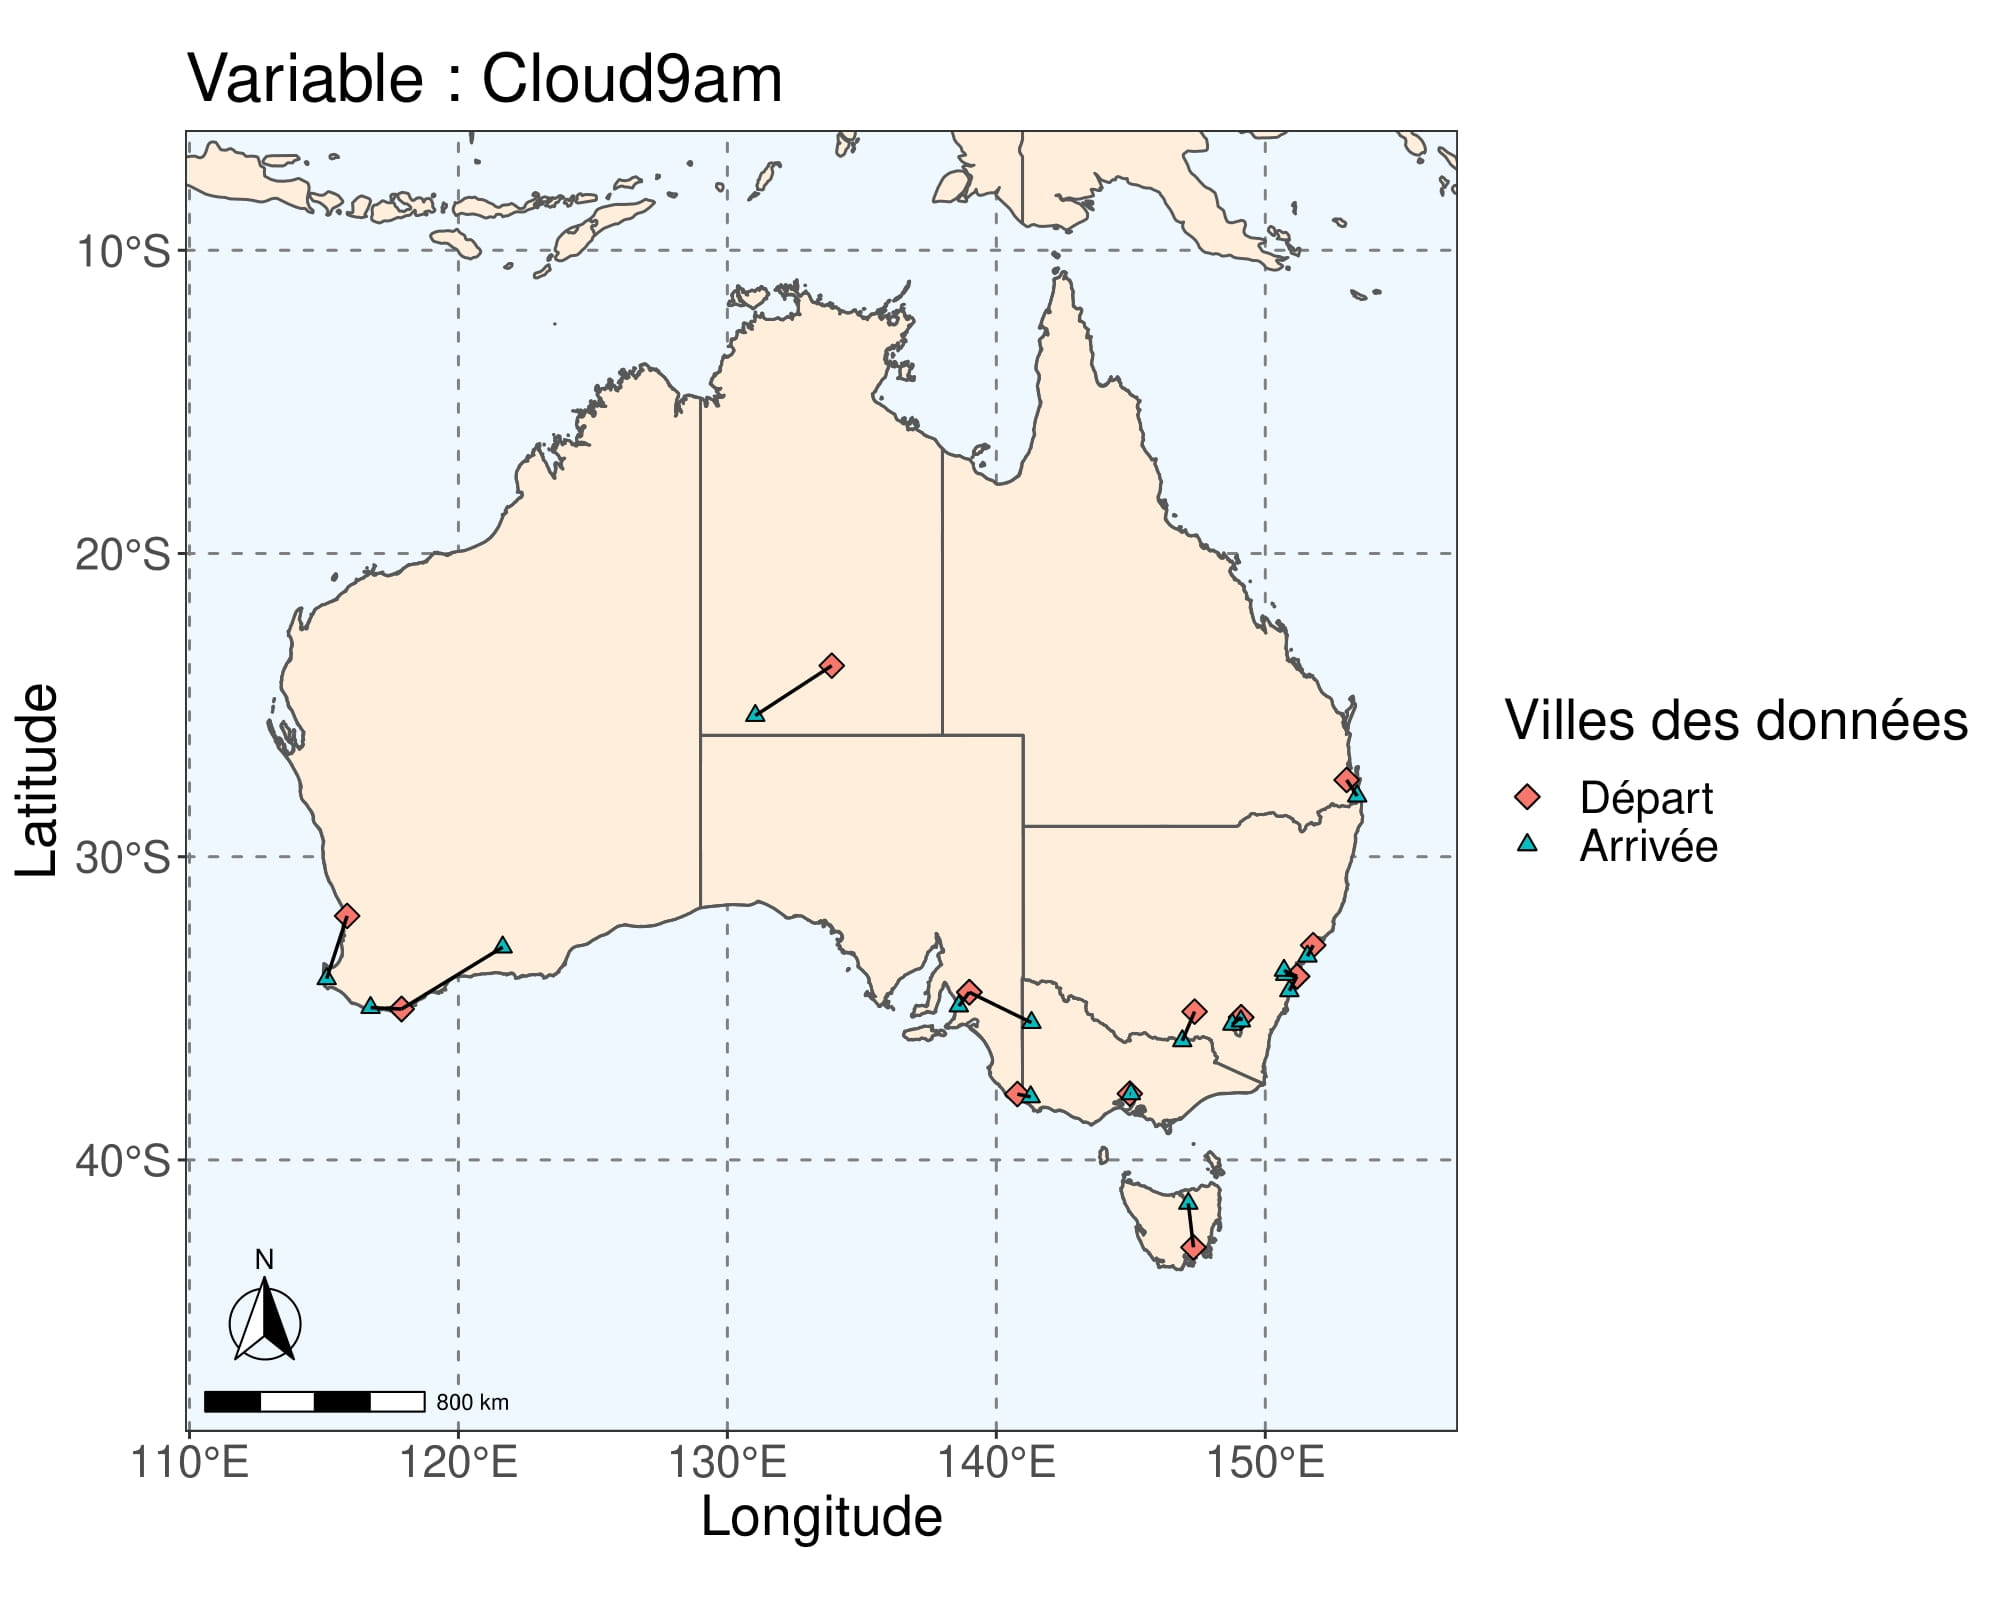
\includegraphics[width=0.48\textwidth]{Images/Australia_map_segments_complete/Australia_map_segments_complete-1.jpg}
    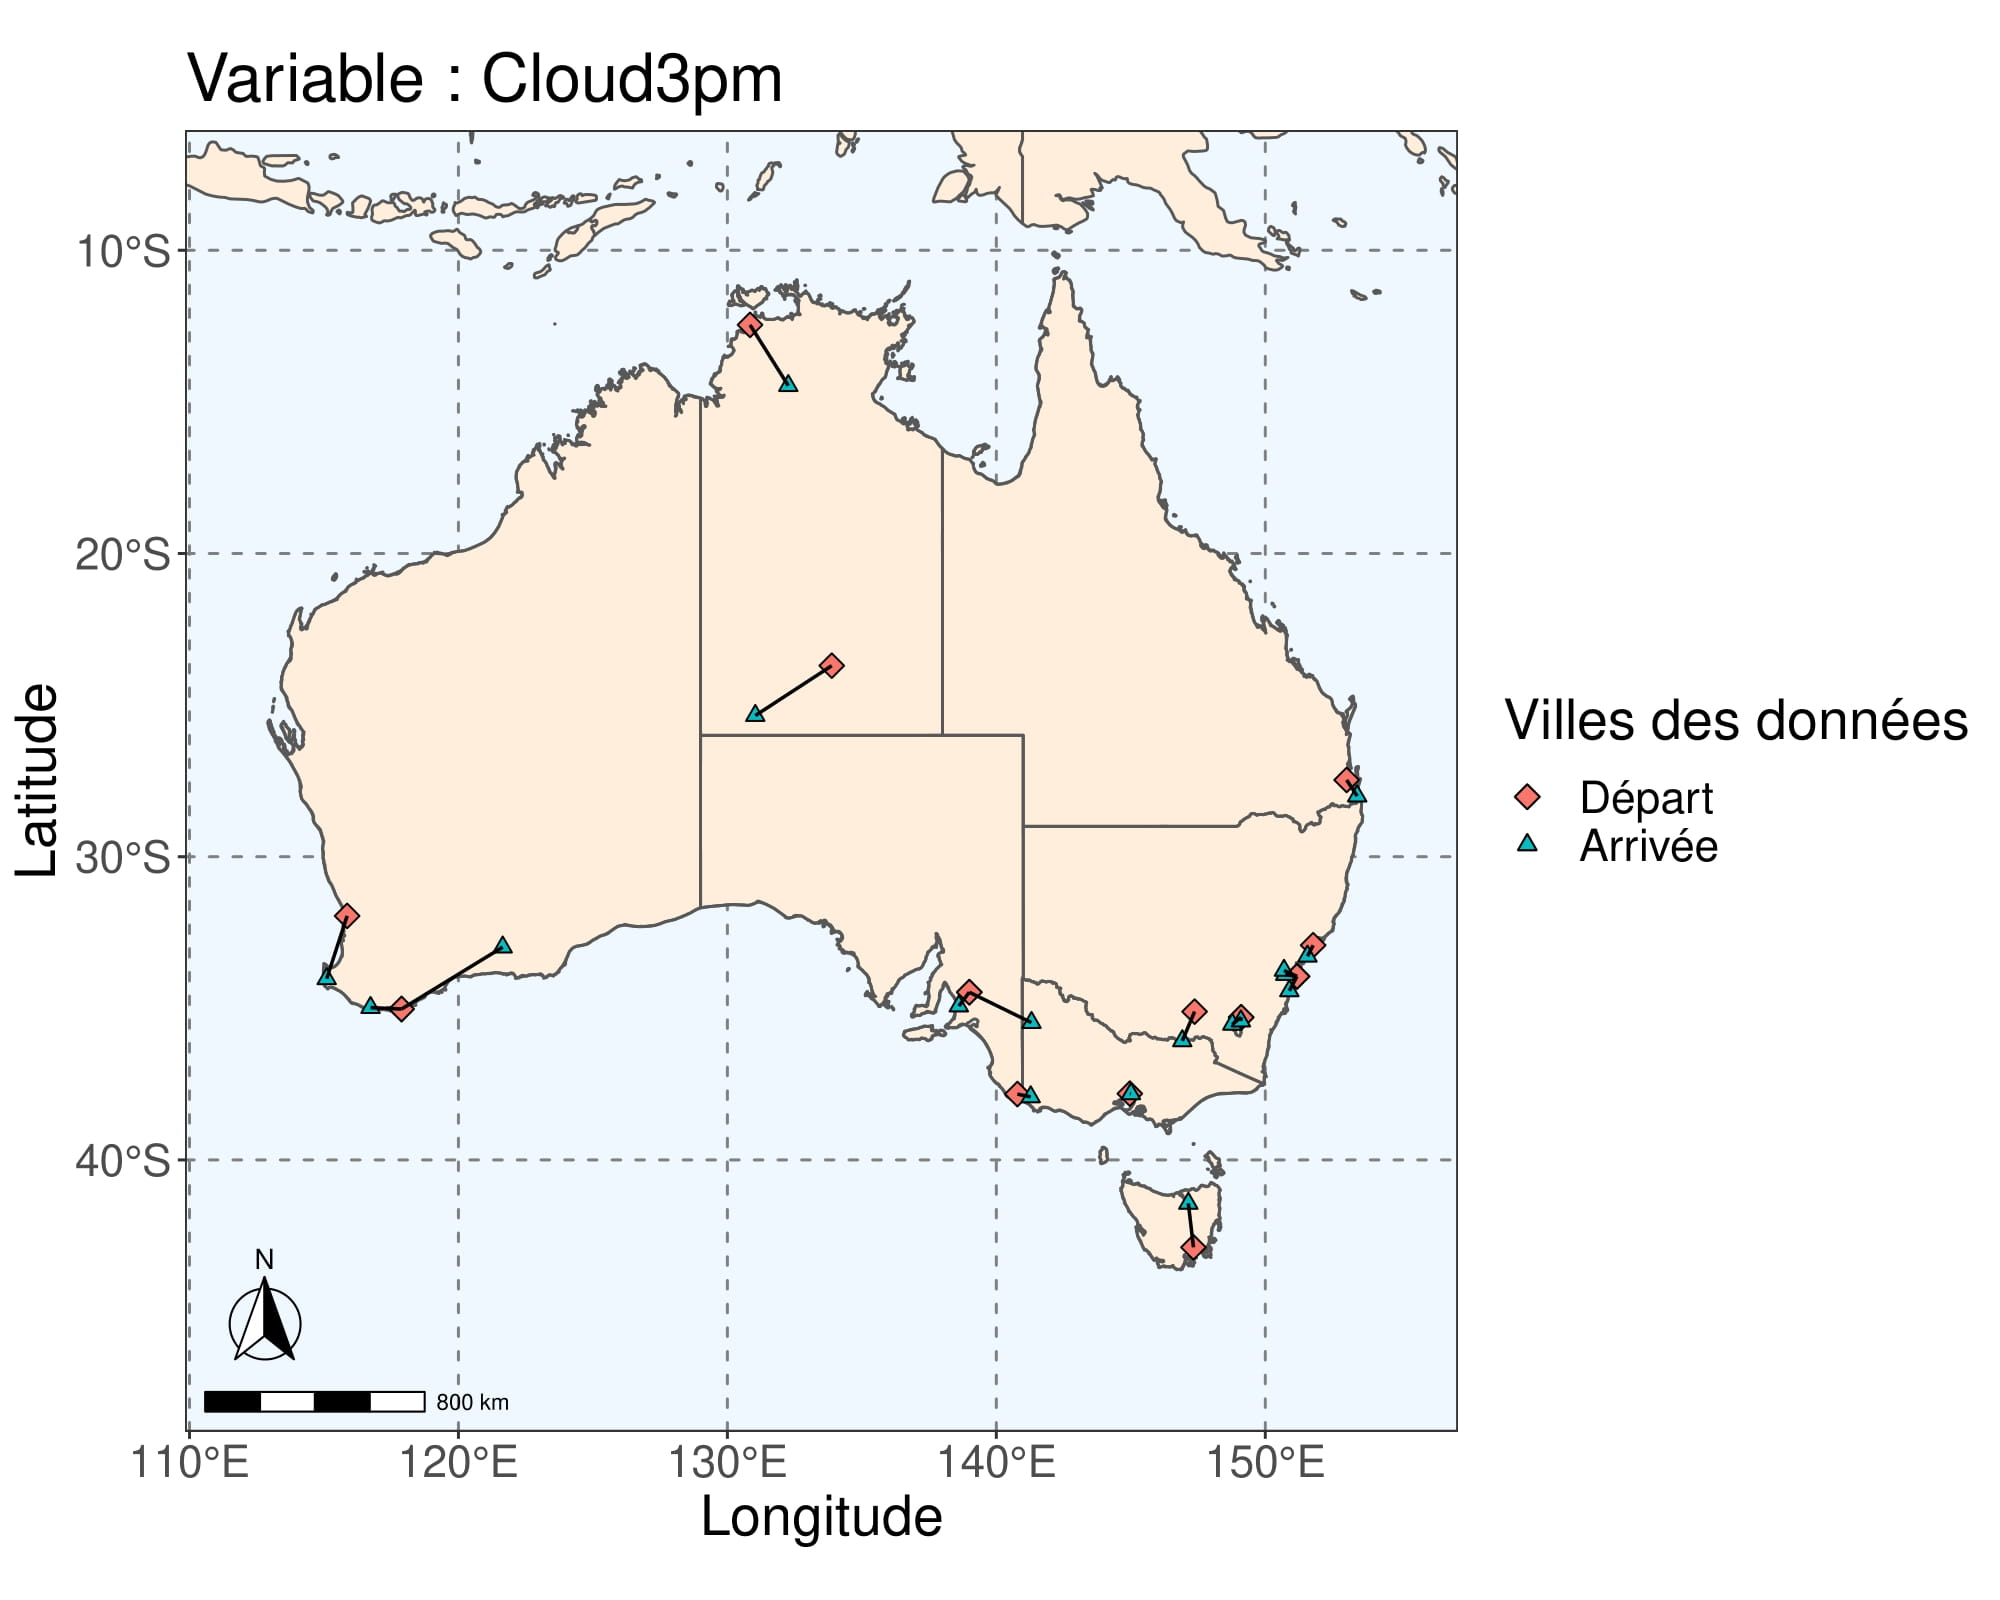
\includegraphics[width=0.48\textwidth]{Images/Australia_map_segments_complete/Australia_map_segments_complete-2.jpg}
    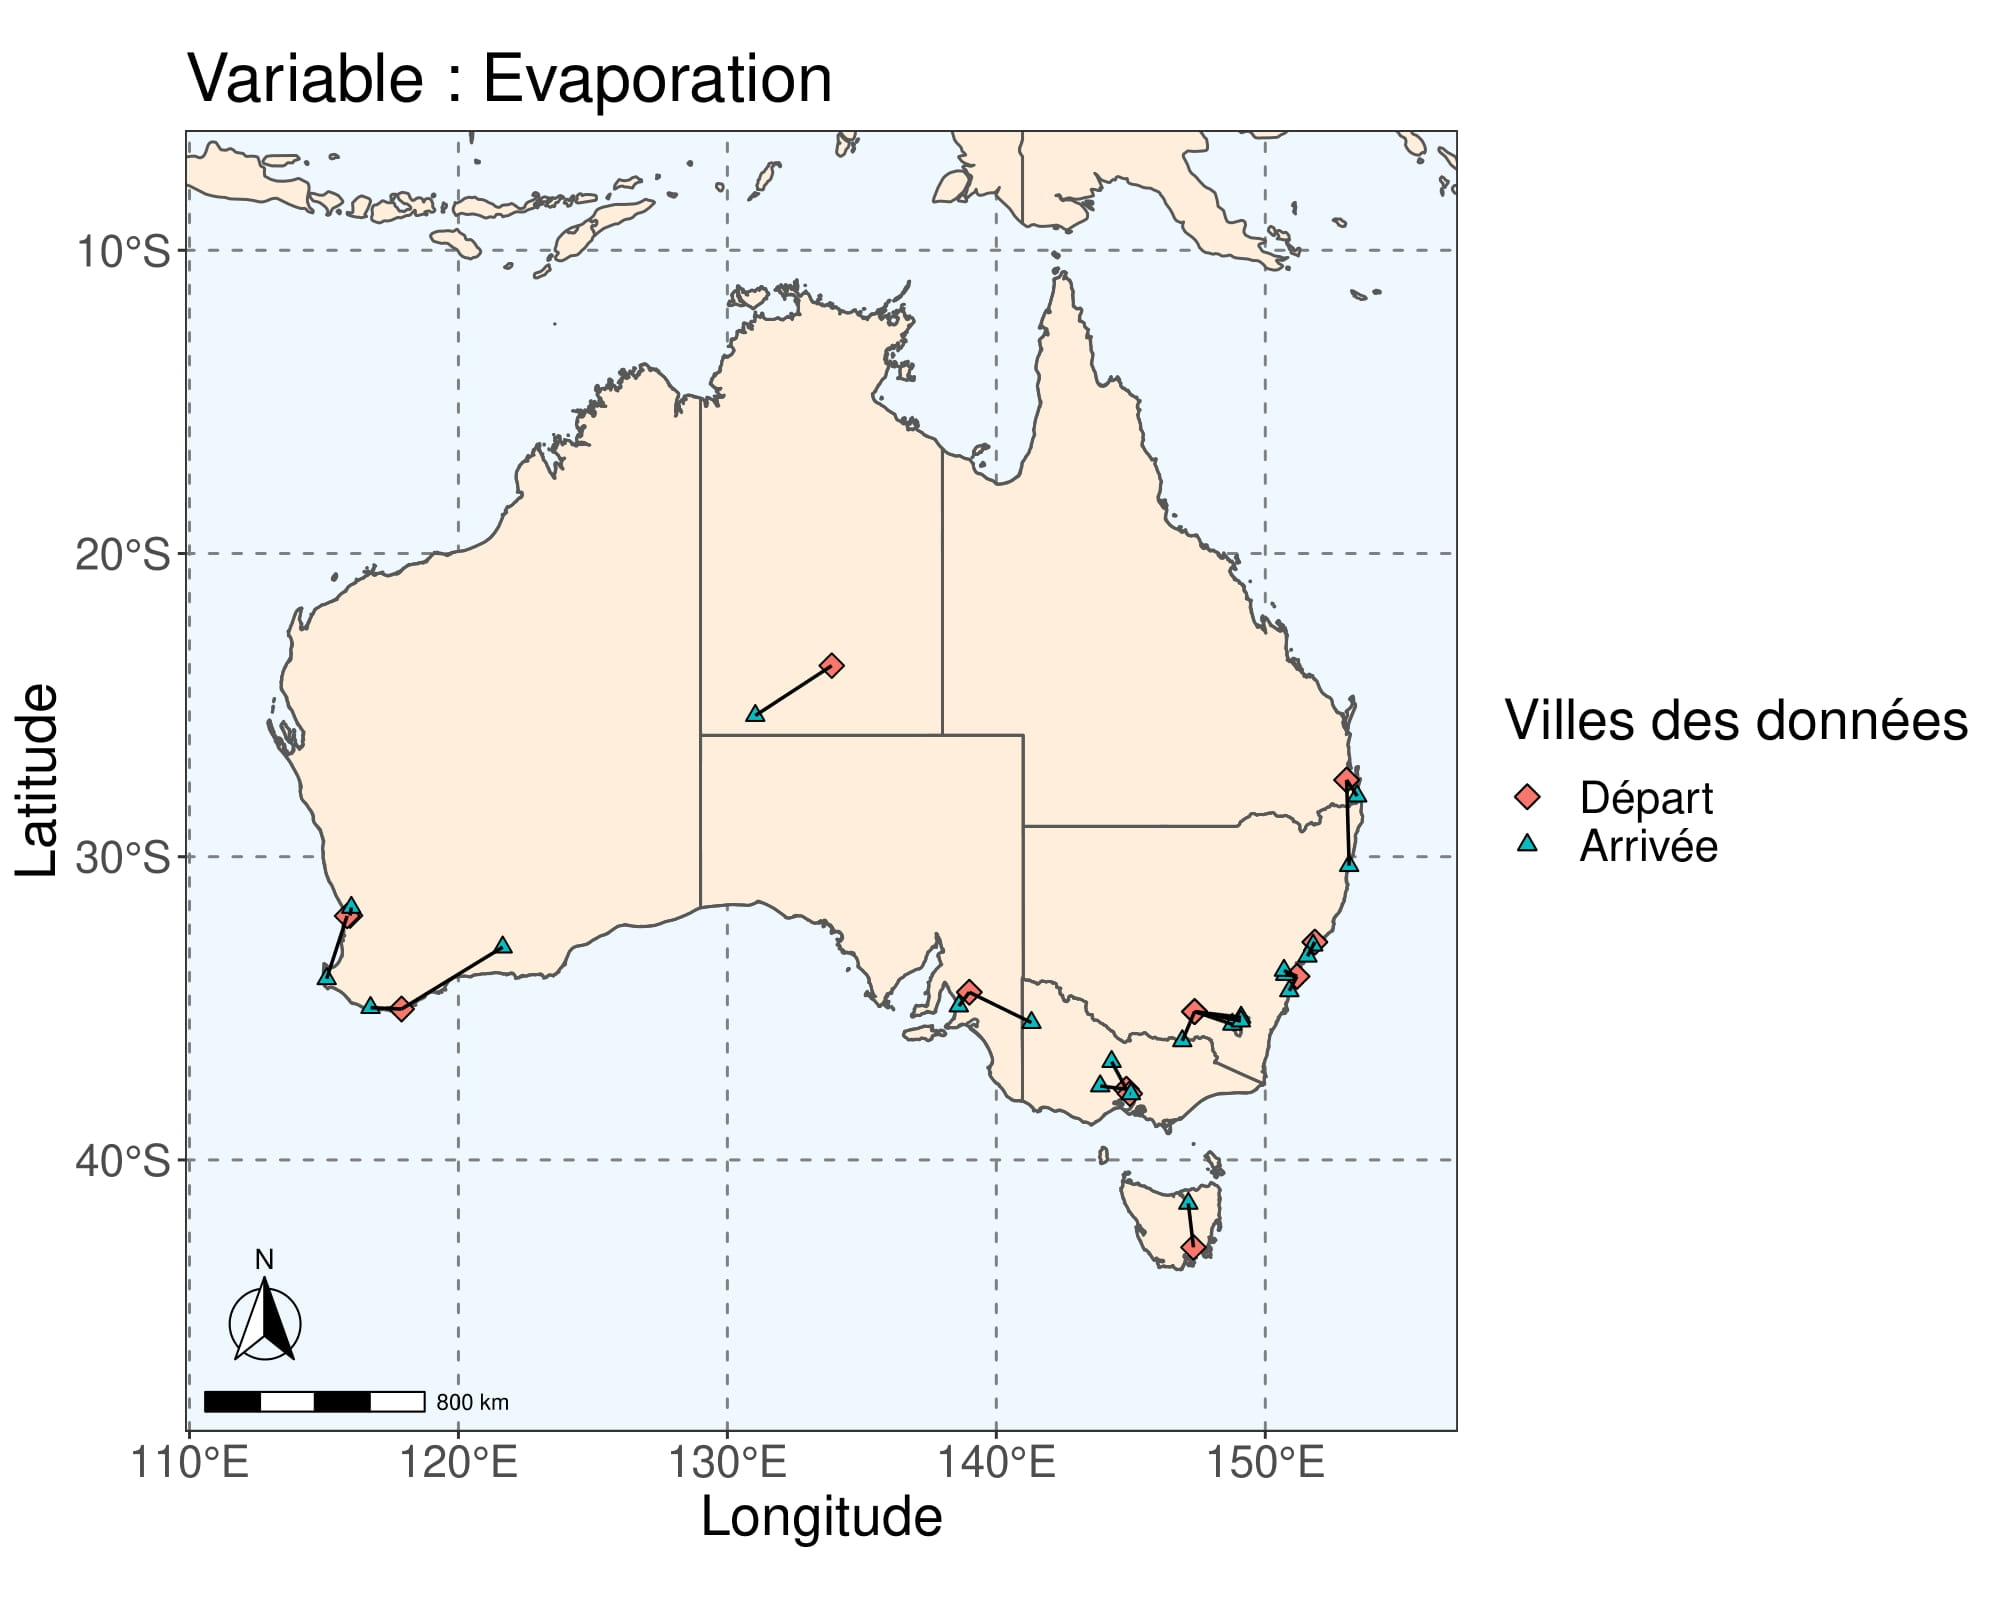
\includegraphics[width=0.48\textwidth]{Images/Australia_map_segments_complete/Australia_map_segments_complete-3.jpg}
    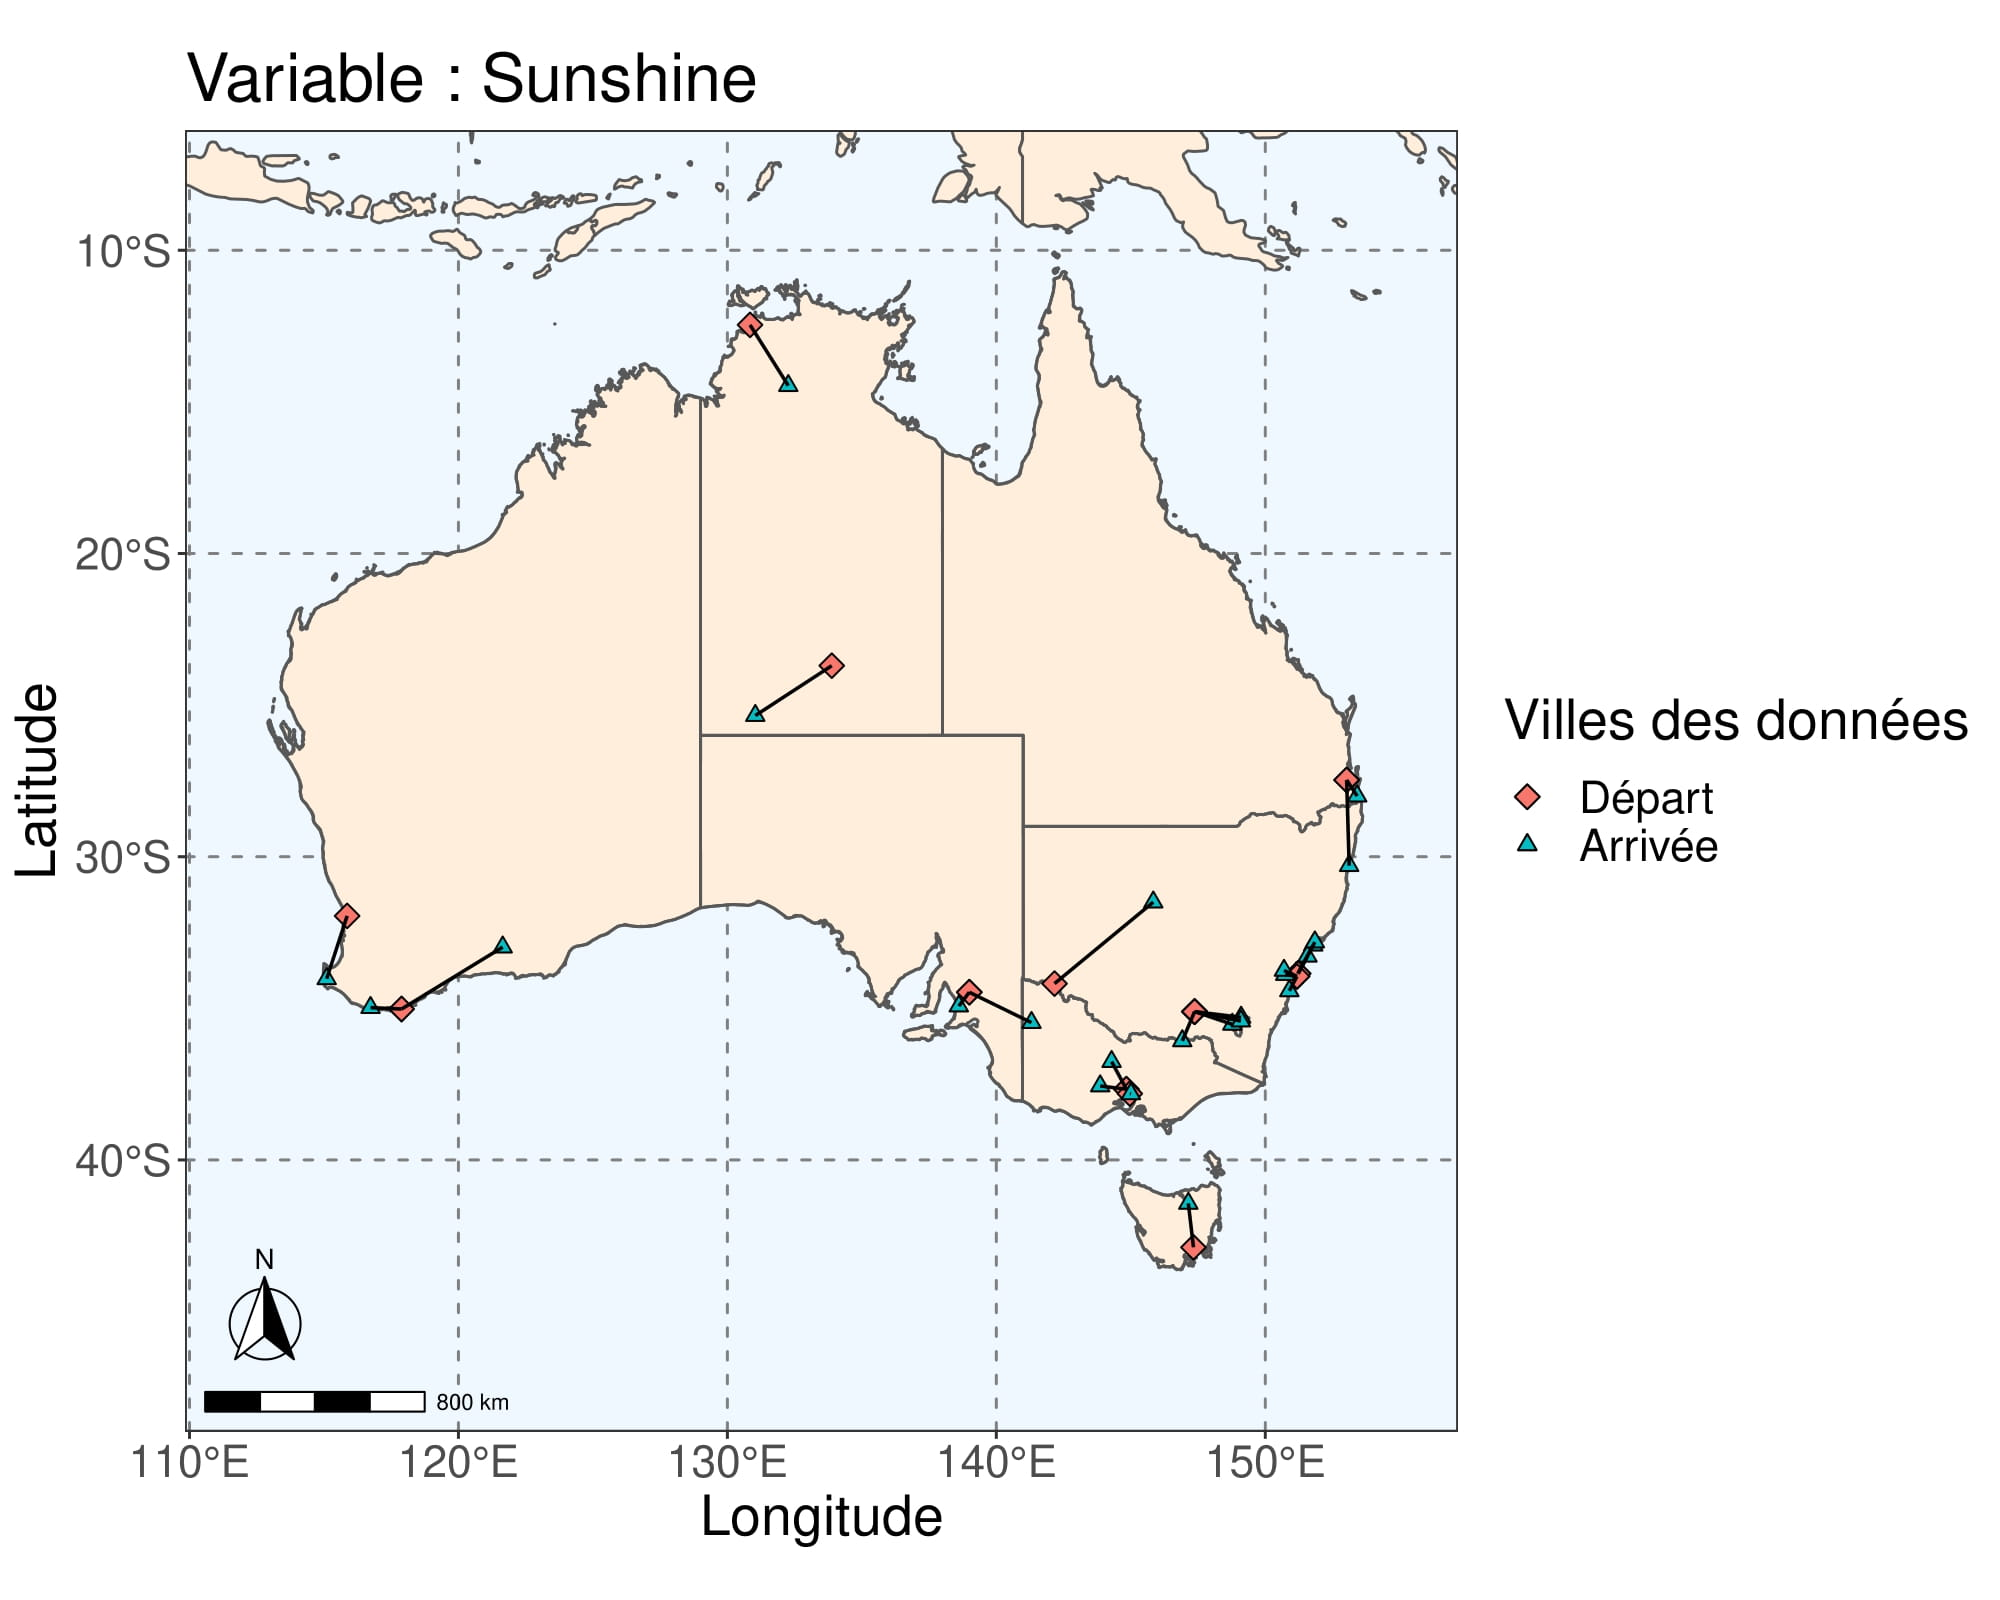
\includegraphics[width=0.48\textwidth]{Images/Australia_map_segments_complete/Australia_map_segments_complete-4.jpg}
    \caption{Chemin des observations copiées (ville de départ et ville(s) d'arrivée(s)) pour certaines des variables complétées.}
\end{figure}

Au final, le \emph{na.omit} nous donne une base de données avec $105546$ observations. La missingness map et la distribution des observations par lieu sont les suivantes : 

\begin{figure}[H]
    \centering
    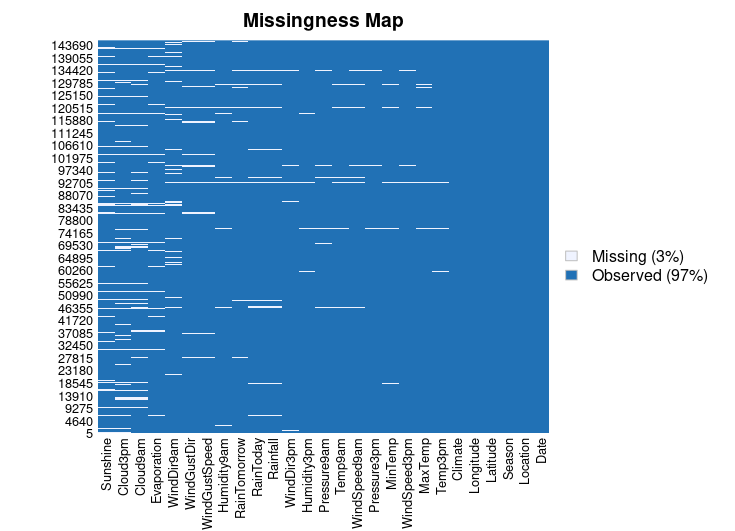
\includegraphics[width=0.7\textwidth]{Images/missmap_completed.png}
    \caption{Missingness Map des données complétées.}
\end{figure}

\begin{figure}[H]
    \centering
    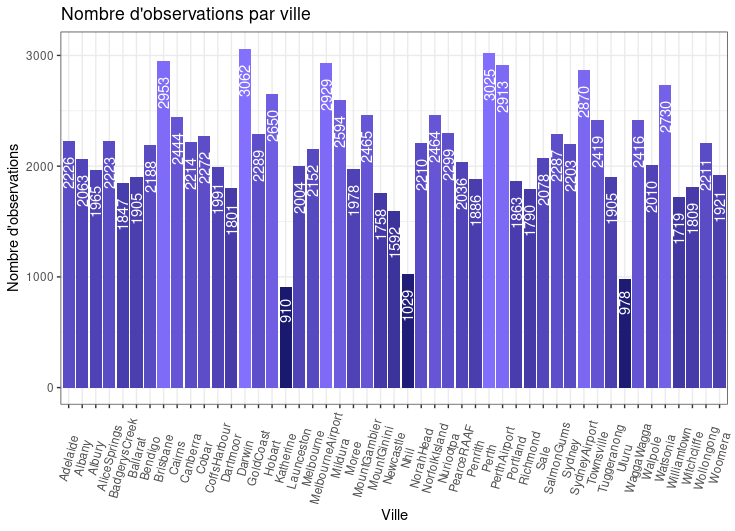
\includegraphics[width=0.7\textwidth]{Images/distribution_lieux_completed.png}
    \caption{Distribution des observations par villes dans notre base de données finale.}
\end{figure}

On remarque que certaines plages de dates n'ont pas été complétées pour certaines variables, il peut y avoir deux raisons à cela : 
\begin{itemize}
    \item Le lieu pour cette variable n'a pas été considéré comme à compléter, malgré quelques valeurs \emph{NA};
    \item Le lieu qui a servi pour la complétion certaines dates en moins que celles du lieu à compléter.
\end{itemize}
Le nombre d'observations de notre base de données finale reste cependant satisfaisante et tous les lieux y sont représentés.

\newpage
\printbibliography

\end{document}
